% 第 10 题椭圆图：按固定源 PDF 矢量路径换算（1 pt → 0.03515 cm）。
% 原点取椭圆中心 O（源页 (220.21, 747.97) pt），y 向上。
% 椭圆半轴 49.08×28.34（b/a=1/√3，源为按题设精确作图），线宽 0.8pt（其余图元 2 倍）；
% x 轴左 −62.33 右至箭头尖点 62.34；y 轴下 −36.83 上至箭头尖点 36.84。
% 弦 y=b/2（过 B、C）、线段 BF/CF、F 处直角记号（三折线）照源；
% O、F 标签在 x 轴下方（源内如此，照录）。
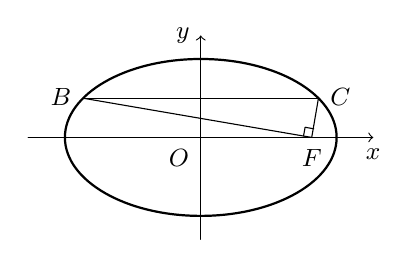
\begin{tikzpicture}[line cap=round,line join=round,font=\small,x=0.03515cm,y=0.03515cm]
% 坐标轴
\draw[->] (-62.33,0)--(62.34,0);
\draw[->] (0,-36.83)--(0,36.84);
% 椭圆（线宽 0.8，与源一致）
\draw[line width=0.8pt] (0,0) ellipse (49.08 and 28.34);
% 弦与焦点弦
\draw (-42.50,14.17)--(42.51,14.17);   % 弦 y=b/2（B–C）
\draw (-42.50,14.17)--(40.08,0);       % B–F
\draw (40.08,0)--(42.51,14.17);        % F–C
\draw (37.13,0.57)--(37.69,3.68)--(40.81,3.12);  % F 处直角记号
% ===== 标注（照源字框中心，显式坐标）=====
\node[anchor=center,inner sep=0] at (-6.49,36.84) {\(y\)};
\node[anchor=center,inner sep=0] at (-50.50,14.73) {\(B\)};
\node[anchor=center,inner sep=0] at (50.47,14.74) {\(C\)};
\node[anchor=center,inner sep=0] at (-7.84,-7.28) {\(O\)};
\node[anchor=center,inner sep=0] at (40.13,-7.30) {\(F\)};
\node[anchor=center,inner sep=0] at (62.26,-5.95) {\(x\)};
\end{tikzpicture}
